\documentclass[11pt,twocolumn]{article}

%
% Eit utval av vanlege pakker. Du kan fjerne dei du ikkje trenger eller la dei stå.
%
\usepackage[utf8]{inputenc} % Tillet blant anna norske bokstavar
\usepackage[T1]{fontenc}
\usepackage[nynorsk]{babel}  % Nynorsk
% \usepackage[norsk]{babel} % Bokmål
\usepackage[]{hyperref} % Hyperlenkjer, legg til hidelinks mellom [] for å fjerna boksar rundt
\usepackage{parskip} % Avsnitt er skilt med mellomrom i staden for innrykk
\usepackage[]{graphicx} % For å inkludere bilete.
\usepackage{physics} % Kjempenyttig pakke! Kort og god manual.
\usepackage[separate-uncertainty=true]{siunitx} % Enkel og riktig formatering av einigar
\usepackage{tikz} % For å teikne eigen vektorgrafikk direkte i Latex(!). Veldig god (og lang) manual.
\usepackage{lmodern} % Bedre fontar
% \usepackage{fancyhdr}
\usepackage{amsmath} % American mathematical society
\usepackage{amssymb}
\usepackage[version=3]{mhchem} % Kjemiske formlar
\usepackage{pgf} % For plotting direkte i Latex(!). Denne brukar tikz i botnen.
\usepackage{pgfplots} % For plotting. For interesserte er manualen veldig god (og laaang).
\pgfplotsset{compat=newest}
\usepackage{pgfplotstable} % For å lese inn tabellar med pgfplots
\usepackage{subcaption} % For å setje fleire figurar side ved side
\usepackage{float} % Forbedring av "flytande objekt" (bilete o.l.)
\usepackage{xcolor} % Definerar mange fargar
\usepackage[section]{placeins} % Forhindrar at flytande objekt flyt forbi seksjonen dei blei definert i
\usepackage[normalem]{ulem} % Fancy underlinjer
\usepackage{gensymb} % Definerar nokre nyttige symbol. F.eks. \degree
\usepackage{mathrsfs} % Kalligrafiske bokstavar
\usepackage[tmargin=20mm, bmargin=20mm]{geometry} % Her kan du velje storleiken på margane
\newcommand{\vect}[1]{\boldsymbol{#1}} % Feit skrift for vektorar.
% \newcommand{\vect}[1]{\vec{#1}} % Pil over bokstav for vektorar.
\DeclareSIUnit\time{t} % Eigen definisjon av einingen time. Hour (h) på engelsk

%
% Her startar dokumentet
%
\begin{document}
%
% Overskrift, forfattar, dato (dette kan gjerast på mange andre måtar og. F.eks \maketitle)
%
\title{FYS103 Rapportmal\\{\large Mal med enkle eksempel for fyrstegongsbrukarar av \LaTeX}}
\date{\today}
%\author{Eivind Seim}

\twocolumn[
\begin{@twocolumnfalse}
  \maketitle
  % slett linjene frå her...
  Dette dokumentet tek sikte på å gje eit eksempel på korleis ein kan
  bruka \LaTeX\ til å generera ein rapport på ein enkel måte. Du kan
  lesa dokumentet parallelt med .tex fila for å sjå korleis ein skriv
  likningar, legg til bilete og anna. Meir detaljert om kva som skal kvar i
  ein rapport finn du i presentasjonen til forelesinga på Canvas.\\

  I botnen av dokumentet finn du ei liste med lenkjer til nyttig
  informasjon for nybyrjaren av \LaTeX -systemet. \vspace{2em}
  % ... til her
  \abstract{Kort samandrag av resultat og konklusjon.}
  \vspace{2em}
\end{@twocolumnfalse}
]
  
\section*{Innleiing}
Skildre fenomenet som skal undersøkjast og motiver forsøket. Du kan
også refere til labheftet \cite{labtext} eller litteratur
\cite{Jackson}.

\section*{Teori og metode}
Presenter kort teorien som ligg til grunn og forklar likningar som
vert brukt til å gjera utrekningar. Metoden skal vere skildra presist
og må inneholda kvar utstyr som blei brukt og korleis ein gjekk fram.

Nokre likningar, sjå kjelden for syntaks. Likning
\eqref{eq:newtonsandrelov} er Newtons andre lov
\begin{equation}
  \vect{F} = m\vect{a} = \frac{\dd{\vect{p}}}{\dd{t}}, % \dd{} er frå physics-pakka. Veldig hendig!
  \label{eq:newtonsandrelov} % bruk merkelappar for å enkelt referere til likningane dine
\end{equation}
og likning \eqref{eq:standardavvik} er standardavviket til ein diskret
stokastisk variabel $x$,
\begin{equation}
  \label{eq:standardavvik}
  \sigma = \sqrt{\frac{1}{n}\sum_{i=1}^n(x_i-\mu)^2}.
\end{equation}

\section*{Resultat og diskusjon}
Her blir resultata presentert og diskutert. Moglege feilkjelder må
drøftast. Bilete/tabellar/grafar/plott (figurar) må ha ein tilhøyrande
figurtekst som gjev ei forklaring så god at teksten og figuren kan stå
uavhengig av resten av rapporten. Figurteksten skal stå under
tilhøyrande figur slik som i Fig. \ref{fig:spektrometer}.
\begin{figure}[tpbh]
  \centering
  \includegraphics[scale=0.25]{spectrometer.jpg}
  \caption{Eit spektrometer.}
  \label{fig:spektrometer}
\end{figure}

Enkle (eller
\href{http://www.texample.net/tikz/examples/area/physics/}{avanserte})
figurar, sjå figur \ref{fig:tikz}, kan teiknast med TikZ og PGFplots
kan plotte enkle (og
\href{http://pgfplots.sourceforge.net/gallery.html}{avanserte}) plott,
sjå figur \ref{fig:pgfplots}.
\begin{figure}[tpbh]
  \centering
  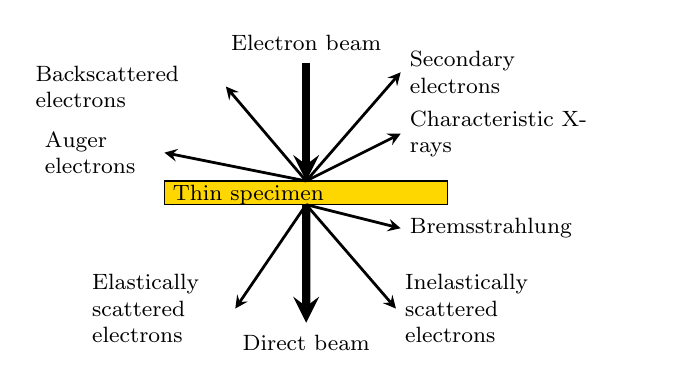
\begin{tikzpicture}[scale=0.6]
    \footnotesize
    \definecolor{ring}{RGB}{255,215,0};
    \coordinate (source) at (3,-0.5);

    \draw[fill=ring] (0,0) -- (6,0) -- (6,-0.5) -- (0,-0.5) -- cycle;
    \draw[-stealth,line width=3pt] (3,2.5) node[above]{Electron beam} -- (3,0);
    \draw[-stealth,line width=3pt] (source) -- (3,-3) node[below]{Direct beam};
    \draw[-stealth,line width=1pt,text width=1.7cm] (source) -- (1.5,-2.7) node[below,left]{Elastically scattered  electrons};
    \draw[-stealth,line width=1pt,text width=2cm] (source) -- (4.9,-2.7) node[below,right]{Inelastically scattered  electrons};
    \draw[-stealth,line width=1pt,text width=2.5cm] (3,0) -- (5,1) node[right]{Characteristic X-rays};
    \draw (0,-0.3) node[right]{Thin specimen}; 
    \draw[-stealth,line width=1pt,text width=1.4cm] (3,0) -- (0,0.6) node[left]{Auger electrons};
    \draw[-stealth,line width=1pt,text width=2.3cm] (3,0) -- (1.3,2) node[left]{Backscattered electrons};
    \draw[-stealth,line width=1pt,text width=2cm] (3,0) -- (5,2.3) node[right]{Secondary electrons};
    \draw[-stealth,line width=1pt,text width=3cm] (source) -- (5,-1) node[right]{Bremsstrahlung};
  \end{tikzpicture}
  \caption{Ein enkel figur i TikZ}
  \label{fig:tikz}
\end{figure}

\begin{figure}[tpbh]
  \centering
  \begin{tikzpicture}[scale=1]
    \begin{axis}[
      small,
      width=7cm,
      ylabel={$y$},
      xlabel={$x$},
      legend style={at={(0,1)}, anchor=north west},
      ]

      \addplot[        
      ]
      table[x=M,y=N] {tboxcount.txt};
      \addlegendentry{Data}

      \addplot[
      red,
      dashed,
      no marks,
      ]
      table[
      x=0,
      y={create col/linear regression={y=1}},
      skip first n=1] {tboxcount.txt};
      \xdef\slopeA{\pgfplotstableregressiona}
      \xdef\interceptA{\pgfplotstableregressionb}
      \addlegendentry{$\pgfmathprintnumber{\slopeA}\,x \pgfmathprintnumber[print sign]{\interceptA}$}
    \end{axis}
  \end{tikzpicture}
  \caption{Eksempel på plott med regresjon.}
  \label{fig:pgfplots}
\end{figure}

Eit tal kan presenterast med siunitx-pakka slik: $\SI{0.58(2)e-4}{\kilo\meter}$. Eller i
ei likning som ein del av ein utrekning:
\begin{equation}
  \frac{s}{t} = \frac{\SI{100}{\kilo\meter}}{\SI{1}{\time}} = \SI[per-mode=symbol]{100}{\kilo\meter\per\time}
\end{equation} % prøv å ta bort [per-mode-symbol] og sjå kva som skjer.

\section*{Konklusjon}
Her skal du dra konklusjonar basert på det som er skildra i resultat- og diskusjonsdelen.

% Dei to neste seksjonane er sjølvsagt ikkje ein del av
% rapporten. Slett frå her...
\section*{Nyttige lenkjer \footnote{Generelt er Google er ein veldig nyttig venn dersom du klarar å formulera spørsmålet ditt rett.}}
\begin{itemize}
  \item{\href{http://www.youtube.com/user/mrskrummel}{Michelle Krummel sine inroduksjonsvideoar til LaTeX}}
  \item{\href{http://www.harding.edu/lmurray/LaTeX_files/Intro_to_LaTeX/Document.pdf}{\textit{Introduction to \LaTeX} av Lambert Murray}}
  \item{\href{http://en.wikibooks.org/wiki/LaTeX/}{\LaTeX på Wikibooks}}
  \item{\href{http://www.tug.org/pracjourn/2006-4/madsen/madsen.pdf}{Matteformatering av Lars Madsen}}
  \item{\href{www.texblog.org}{TexBlog}}
  \item{\href{http://tug.org/}{\TeX Users Group}}
\end{itemize}

\section*{Installasjon}
Du kan bruka \LaTeX\ på mange måtar. Du kan installera systemet lokalt
på eigen datamaskin eller bruke ein webapp, f.eks
\href{www.overleaf.com}{Overleaf} (før Sharelatex). Overleaf er veldig
hendig når ein skal samarbeide med andre om å laga ein
rapport. Gruppesjefen lagar eit prosjekt som vert delt med dei andre
på gruppa. Alle treng ein brukarkonto, men ingen treng installere
noko.

Ein anna metode er å installera ein \LaTeX\ distribusjon og gjere
redigeringa i ein dedikert editor eller teksthandsamar. Det er
frykteleg mange å velja mellom, men
\href{https://tex.stackexchange.com/questions/339/latex-editors-ides}{denne}
sida lister opp mange.

Anbefalt til nykommaren:
\begin{itemize}
  \item Windows:
    \begin{itemize}
      \item Distribusjon: \href{https://miktex.org}{MiXTeX}, \href{http://www.tug.org/texlive/}{TeX Live}
      \item Editor: \href{http://www.texniccenter.org}{TeXnicCenter}, \href{http://www.xm1math.net/texmaker/}{TeXMaker}
    \end{itemize}
  \item MacOS:
    \begin{itemize}
      \item Distribusjon: \href{http://www.tug.org/mactex/}{MacTeX}
      \item Editor: \href{http://pages.uoregon.edu/koch/texshop/}{TeXShop}
    \end{itemize}
  \item GNU/Linux:
    \begin{itemize}
      \item Distribusjon: Installer \href{http://www.tug.org/texlive/}{TeX Live} frå pakkebrønnen til din distro
      \item Editor: \href{http://www.xm1math.net/texmaker/}{TeXMaker}
    \end{itemize}
\end{itemize}

Du kan spørre om meg på eise@nmbu.no for hjelp til installasjon dersom
du trenger det.
% ... til her

% Du kan bruka bibtex til å handtere referansar
% Legg referansane inn i fila referansar.bib
% For at dokumentet skal kompilere riktig må du køyre pdflatex,
% bibtex, pdflatex, pdflatex. Mange editorar gjer dette automatisk for deg.
\bibliographystyle{plain}
\bibliography{referansar.bib}



\end{document}
%%% Local Variables:
%%% TeX-command-extra-options: "-shell-escape"
%%% mode: latex
%%% TeX-master: t
%%% End:
